\subsection{Problem 3 - Inequality Constrained Quadratic Programming}
From page 475 in Nocedal and Wright the following system is given.
\begin{equation}
\begin{split}
\min_{x} q(x) = (x_1-1)^2+(x_2-2.5)^2 \\
s.t. x_1-2x_2+2> = 0,\\
-x_1-2x_2+6>=0,\\
-x_1+2x_2+2>=0,\\
x_1>=0,\\
x_2>=0.
\end{split}
\end{equation}
in MatLab a contour plot of this is made and seen in figure~\ref{fig:exe3_contour_plot}.
\begin{figure}[H]
	\centering
		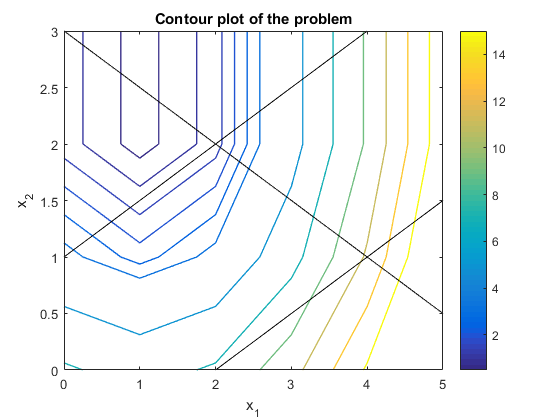
\includegraphics{exe3_contour_plot.png}
	\caption{A contour plot of the problem.}
	\label{fig:exe3_contour_plot}
\end{figure}
From the constrain lines it is seen that the feasible region is a pentagon starting from the origin.\\
The problem can be written in the standart martix way as:
\[H=\begin{bmatrix}
	2 & 0 \\0 & 2
\end{bmatrix}\]
\[g=\begin{bmatrix}
	-2 \\-5
\end{bmatrix}\]
\[A=\begin{bmatrix}
	1 & -1 & -1 & 1 & 0 \\
	-2 & -2 & 2 & 0 & 1
\end{bmatrix}\]
\[b= \begin{bmatrix}
	-2 \\-6 \\-2 \\0 \\0 \\
\end{bmatrix}\]
Then the general KKT system can be written as:
\[\begin{bmatrix}
	H & -A \\A^T & 0
\end{bmatrix}\times
	\begin{bmatrix}
		x\\ \lambda
	\end{bmatrix}=
		\begin{bmatrix}
			-g\\ b
	\end{bmatrix}\]
When the system can be solve with the same QP solver as used for problem 1. That gives:
\[x=\begin{bmatrix}
	-2 \\ 0
\end{bmatrix}\]

\[\lambda=\begin{bmatrix}
	0 \\1.8 \\-0.3 \\-2.1 \\ 3.0
\end{bmatrix}\]
Where all the values are multiply with 10 in the power of 16. 
\\A way to found the optimal solution is with an active set algorithm. This is applyed as the one in the Example 16.4 in N and W. The algorithm is seen in the MatLab code and the contour plot with the four different workingset are seen in figure \ref{fig:exe3_contour_plot_workingset} below. 
\begin{figure}[H]
	\centering
		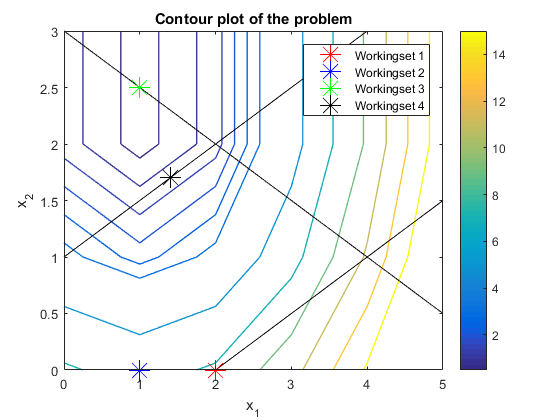
\includegraphics[scale=0.65]{exe3_contour_plot_workingset.png} 
	\caption{A contour plot of the problem, with the working set applyed.}
	\label{fig:exe3_contour_plot_workingset}
\end{figure} 
In figure \ref{fig:exe3_table_part5} below, values for the iteration are shown. 
\begin{figure}[H]
	\centering
	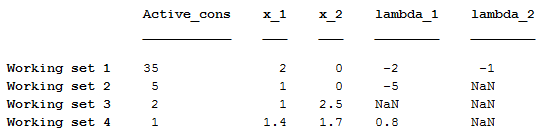
\includegraphics[scale=1]{exe3_table_part5.png} 
	\caption{Table from MatLab showing values from the four iterations.}
	\label{fig:exe3_table_part5}
\end{figure}
From the figure it is seen that for the first working set, constrain 3 and 5 where active. This set found the point (2;0) at the contour plot it is seen that this point is feasible, but that it is not the optimal solution. This is also seen from the Lagrange multipliers, $\lambda$, where they both are negative which they don't are for the optimal solution. \\The next step was to chose a new working set, since the first have two active constrains one of them was remove. Here the 'rule of thumbs' says that the constrain with the most negative Lagrange multipliers should be inactive. There for working set 2 have the 5th. constrain active. This iteration gives the solution (1;0) and $\lambda$ = -5. Since the Lagrange multiplier still is negative, the point is not the optimal solution, this is also confirmed from the contour plot. \\The 3th. step is, again, to remove the constrain belong to the most negative Lagrange multiplier. In this case there are only one, this means that the third working set doesn't have any active constrains. In that case there wouldn't  be any Lagrange multipliers since they 'belongs' to the constrains. The point found in is iteration was (1;2.5). Since there are no Lagrange multiplier the point is inserted in the 'original' constrains which all of the should be equal ore bigger than zero. From the first constrain it is seen that it gives -2 which mean that the constrain is not full fill and therefor not a solution to the problem. From the contour plot it is seen that the point is in the center (if it doesn't have any constrain), but it is also seen that the point is beyond one of the constrain and there for confirm that the found point is not a solution.\\Finally the last working set is chosen to be the first constrain since it was this one there was not full fill. This give the point (1.4;1.7) and $\lambda$ = 0.8. Since the Lagrange multiplier is positive it could be an optimal solution, there for all the constrain are controlled with the found point. It is seen that they give; 0, 1.2 and 4 for the first three constrain, and since constrain four and five are the $x_1$ and $x_2$ bigger ore equal zero they are also full fill. This mean that the found solution is valid and the Lagrange multiplier indicate an optimal solution. This is finally verified by the contour plot where it is easy seen that the point is the global minimum, and the problem is solved. \\
\\
		EXPLAIN THE ACTIVE SET METHODE!!
\\
\\For the active set method to work, an feasible starting point is needed. A good way to found such a point is by using the MatLab function linprog. This is done and can be seen in the MatLab code. This calculate a feasible point (2.47;1.12). In figure \ref{fig:exe3_contour_plot_linprog} below, the found point is seen, and it is seen that it is feasible as expected.
\begin{figure}[H]
	\centering	
	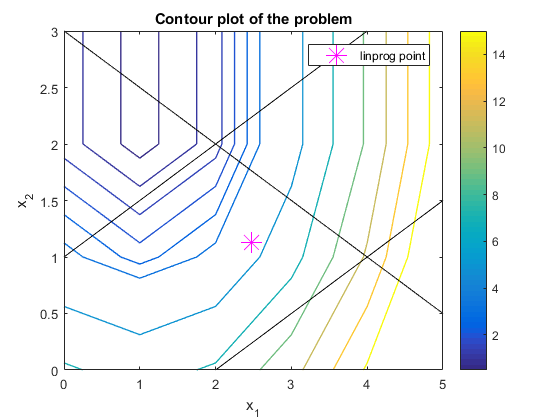
\includegraphics[scale=0.65]{exe3_contour_plot_linprog.png} 
	\caption{The contour plot with the feasible starting point found with linprog.}
	\label{fig:exe3_contour_plot_linprog}
\end{figure}

Finally the entire problem could have been solve using the MatLab program quadprog. This function only needs the matrix H and A,  the vectors g and b, some boundaries and a feasible starting point. By inserting the feasible starting point found with linprog, and the system in the form og H,g A and b. The function found the optimal solution to be (1.4;1.7). Is is consistent with the one found from the active set algorithm, and seen in the contour plot as 'working set 4' in figure \ref{fig:exe3_contour_plot_workingset}.
